\chapter[Introdução]{Introdução}

\section{Contexto}
A tecnologia tem vindo a evoluir rapidamente e, com isto, nota-se o surgimento de
diversos desafios. Um destes desafios é a falta de programadores que possuam competências 
e qualificação necessárias para solucionar os mais diversos problemas presentes nos mais
variados projetos. Este fato está relacionado com a metodologia adotada no ensino de
programação e também com a falta de motivação por parte dos estudantes \cite{7975788}.
\citeonline{inproceedings} afirmam que, uma das razões de os alunos não absorverem eficientemente
os conceitos relacionados à programação se dá pela falta de concentração e motivação dos mesmos frente
a exposição destes conteúdos na forma tradicional.

\citeonline{funcional} destaca que a aprendizagem dos conceitos e mecanismos envolvidos na construção de programas não é
trivial, uma vez que requer a utilização de raciocínio na sua forma mais abstrata. Um dos problemas mais comuns segundo os autores
são: dificuldades no entendimento de comandos, sintaxe dos comandos, dificuldades em entender os resultados da execução de um determinado 
comando pela máquina, dificuldades em dar os primeiros passos relativos ao estudo de programação entre outros.

\citeonline{ambap} diz que, em geral, os alunos têm grandes dificuldades em compreender e aplicar os conceitos relativos à programação . Uma das grandes 
dificuldades está relacionada a problemas de compreensão e aplicação de noções básicas, como por exemplo o uso de estruturas de controle e estruturas
condicionais.

Dificuldades como estas apresentadas, encorajam o desenvolvimento de soluções que auxiliem no ensino e aprendizagem de programação de forma diferente ao
atual modelo de ensino. Diversas abordagens de ensino são estudadas para facilitar o aprendizado dos alunos, algumas delas são:
gamificação, programação imperativa, programação funcional e etc. Neste trabalho, é abordado o uso da gamificação na construção de uma ferramenta
de apoio ao ensino e aprendizagem de programação desenvolvida com base nos requisitos identificados a partir da interação com ex alunos
da disciplina de Algoritmos de Programação de Computadores, ofertada pela Universidade de Brasília, campus Gama.

Segundo \citeonline{6624228}, jogos bem projetados representam bons motivadores, uma vez que passa a sensação de satisfação
e recompensa fazendo com que os jogadores persistam e fiquem engajados em realizar sua missões. Neste contexto, este poder
motivacional dos jogos, passou a ser utilizado em outros contextos que não estão relacionados diretamente aos jogos, uma prática 
conhecida atualmente como Gamificação do inglês \textit{gamification} {\itshape}.

Para \citeonline{Deterding:2011:GDE:2181037.2181040}, o termo gamificação pode ser definido como a utilização de elementos e mecânica de 
jogos em contextos não relacionados a jogos. De acordo com \citeonline{Brazil} a utilização destes elementos tornam tarefas reais em atividades
mais atrativas e lúdicas e, consequentemente, aumentam a motivação e engajamento. Há uma grande variedade de ambientes que possuem 
elementos semelhantes a características de jogos, muitos deles contendo: sistema de pontuação, feedbacks constantes e 
etc \cite{6624228}. São exemplos de ambientes com características semelhantes a de jogos: Uri, Datacamp, Edx entre outras.

A aprendizagem baseada na gamificação, preocupa-se em utilizar de mecanismos de jogos não para o entretenimento,
mas para o ensino. Os interessados no campo da gamificação trabalham para identificar o cenário e as condições 
que possam apoiar a integração de jogos aos ambientes de aprendizado. Vários cientistas e estudiosos no campo
da gamificação apontaram uma diversidade de elementos de jogos que permitem que eles sejam utilizados como
ferramentas de apoio ao aprendizado. Por exemplo: os jogos são bastante envolventes \cite{Dickey2005} e motivadores \cite{Prensky:2003:DGL:950566.950596}. Além destas características,
jogos são excelentes fontes para se adquirir experiência que são dificeis de serem fornecidas por meio de instruções tradicionais \cite{Arena2014}.

Os ambientes online gamificados de apoio ao ensino podem fornecer diversas ferramentas, entre elas: classificações, batalhas, fórums de discussões e etc.
De forma a incentivar os usuários a participarem das atividades propostas. 
Durante as competições e batalhas, os estudantes têm a possibilidade de aprender com outros jogadores e comparar suas habilidades, tornando o aprendizado mais
prazeroso \cite{LearningProgramming}. 

\pagebreak

\section{Justificativa}
De acordo com \citeonline{de2009visualg}, a abordagem de ensino tradicional de programação, que é aquela onde o professor apresenta
uma série de conceitos aos alunos e os mesmos têm a tarefa de entender como se aplicam na resolução de problemas,
para a maioria dos estudantes, se revelam muito abstratas.

Em seu trabalho de conclusão de curso pela Universidade de Brasília , campus Gama (FGA), \citeonline{calixto} apresenta uma pesquisa 
baseada nos dados referentes aos índices de aprovação, trancamento e reprovação dos alunos na disciplina de computação básica (atualmente
a disciplina recebe o nome de Algoritmos e Programação de Computadores, ofertada no campus Gama). 

Os dados utilizados por \citeonline{calixto}, são referentes a um total de 60 turmas e 3286 alunos matrículados nas disciplinas de Computação Básica entre
os anos de 2009 e 2013. Segundo o autor, dos 3286 alunos matriculados, 1659 alunos (50,48\%) foram reprovados, 262 alunos (8\%) trancaram
a disciplina e apenas 1364 alunos (41,5\%) obtiveram aprovação. O autor ainda explica que esses resultados, quando comparados à média nacional de 
aprovação de alunos em disciplinas de programação são bem preocupantes, a taxa apresentada como média nacional é de cerca de 67\% de aprovação, ou 
seja, a taxa de aprovação na FGA, é mais de 30\% menor em relação a média apresentada (67\%).

Contando com a cooperação dos funcionários da secretaria da FGA, obteve-se dados atuais referentes às aprovações, reprovações e trancamentos dos
alunos entre os períodos 2017/1 e 2019/1. Ao analisar estes dados, notou-se que do total de alunos matriculados (2225 alunos divididos em 37 turmas) no decorrer
de 5 semestres, 890 alunos (40\%) foram reprovados, 112 alunos realizaram o trancamento (5\%) e apenas 1223 alunos foram aprovados (54,96\%). Estes dados são preocupantes 
e demonstram a atual situação do aprendizado dos alunos na disciplina de Algoritmos e Programação de Computadores na FGA.

Um estudo realizado pela Universidade Federal da Paraíba (UFPB) que analisou por seis períodos 
acadêmicos os índices de reprovação na disciplina de Introdução à programação, apontou que 
em nenhum dos seis períodos analisados houvera um índice de aprovação superior a 34\%. Além disso,
os índices de reprovação e trancamento da disciplina giraram em torno dos 64\% e 6\% respectivamente \cite{SBIE6739}.

Um outro estudo, realizado na Faculdade de Educação Tecnológica do Estado do Rio de Janeiro (FAETERJ-Paracambi) por \citeonline{vieira2015dificuldades}, 
envolvendo 663 alunos da disciplina de Algoritmos 1 mostrou que, destes alunos, apenas 511 cursaram a disciplina 
até o final, ou seja, cerca de 152 alunos desistiram da disciplina. Do total restante (511), apenas 30\% foram
diretamente aprovados (cerca de 153 alunos), 40\% foram reprovados diretamente (204 alunos) e 30\% foram para o exame final (recuperação, 153).
Dos 153 alunos que foram para a recuperação, apenas 55\% foram aprovados (84 alunos), nota-se então que, dos 663 alunos que
foram matriculados na disciplina, apenas  288 alunos foram aprovados ao seu término, cerca de 43\%.

\section{Problema}
Como desenvolver uma ferramenta gamificada para apoiar o ensino e aprendizagem de programação.
% Nas seções anteriores, apresentou-se alguns estudos realizados a respeito da situação encontrada durante as análises iniciais do ensino e aprendizagem
% de programação em matérias introdutórias, a partir destes panoramas, o presente trabalho, visa demonstrar os resultados e passos dados na construção de uma
% ferramenta gamificada para auxiliar o ensino e aprendizagem de programação.
 
\section{Objetivos}
Desenvolver uma ferramenta gamificada para apoiar o ensino e aprendizagem de programação.

% Tendo sido apresentado o contexto e problema, o objetivo geral do presente trabalho é demonstrar o desenvolvimento e resultados
% obtidos durante a construção da mesma.

% Para alcançar o objetivo geral, foram definidos os seguintes objetivos específicos:
% \begin{itemize}
% 	\item Desenvolvimento da ferramenta gamificada com base nos requisitos;
% 	\item Definição do método de coleta de dados a respeito da utilização da ferramenta pelos usuários;
% 	\item Análise dos dados a respeito da experiência de uso.
% \end{itemize}

\chapter{Referencial teórico}

\section{Aprendizagem de programação}
De acordo com \citeonline{KOLIVER}, disciplinas introdutórias de programação são, em sua maioria, problemáticas e costumam apresentar
altos índices de desistência e reprovações. Um dos motivos para tal ocorrência se dá pela falta de preparo que se espera que alunos
ingressantes nestas disciplinas possuam.

Disciplina de algoritmos são normalmente oferecidas no início da grade curricular dos cursos. Isso faz com que a maioria dos alunos
cursantes sejam calouros que ainda estão acostumados com a forma ``mecanisada'' de ensino que os habituam a somente aplicar fórmulas 
sem qualquer tipo de análise mais profunda dos problemas \cite{KOLIVER}.

De acordo com \citeonline{Borges}, o modo tradicional de ensino (figura \ref{figura4}) não é suficiente para motivar os alunos a se
interessarem por disciplinas de programação. Não fica claro para a maioria dos alunos, principalmente para aqueles
não possuem nenhum tipo de conhecimento em informática, a importância de certos conteúdos.

\begin{figure}[h]
	\centering
	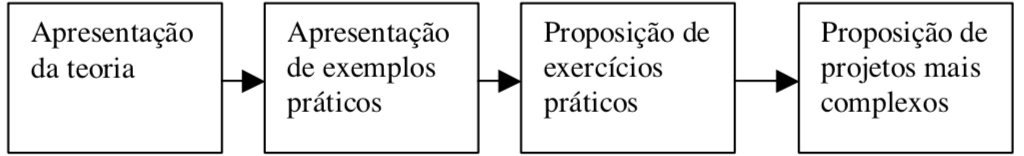
\includegraphics[keepaspectratio=true,scale=0.34]{figuras/modoTradicional.png}
	\caption{Sequência de passos típicos na apresentação de uma disciplina}
	Fonte: \cite{Borges}
	\label{figura4}
\end{figure}

Ao se apresentar uma nova liguagem de programação, é comum as aulas serem realizadas em laboratórios com
recursos computacionais. Apesar dessas aulas apresentarem um formato diferenciado em relação ao modo tradicional,
os professores não exploram a diversidade dos equipamentos disponíveis com práticas que apoiem o desenvolvimento 
de habilidades por parte dos estudantes \cite{Borges}.

\section{Gamificação}
Jogos são uma construção humana que envolvem em seu contexto fatores sociais, culturais e econômicos \cite{EaDF440}.
Como apresentado no livro ``Gamificação na Educação'' por \citeonline{da2014gamificaccao}, a interação com \textit{games}, apesar
dos custos altos dos consoles, foram ocupando cada vez mais o tempo das pessoas que notaram que os jogos poderiam ser boas fontes
de prazer e entretenimento.

O notável crescimento do mercado dos \textit{games} tem atraido diferentes olhares de estudiosos que se dedicam ao estudo de seu
uso na educação, comunicação, marketing, psicologia, computação, entre outras áreas \cite{da2014gamificaccao}.

O termo gamificação, segundo \citeonline{da2014gamificaccao}, consiste na utilização de elementos de jogos em 
atividades que por natureza de sua criação não são jogos. \citeonline{raposo2016desafio} dizem que o objetivo da gamificação, consiste em resolver
problemas práticos ou despertar interesse e engajar um público específico para a realização de uma determinada
atividade. 

Para \citeonline{chou2017actionable}, a gamificação é uma arte que é capaz de derivar elementos divertidos e envolventes encontrados em jogos e utiliza-los
em outras atividades. Para o autor, o foco deve estar centrado no ser humano e na sua motivação.

\subsection{Gamificação na Educação}
Embora o termo gamificação tenha sido apresentado pela primeira vez em 2010, a idéia de se utilizar
elementos de jogos em atividades que não são jogos, tem sido utilizado há muito tempo. Na educação
de crianças, por exemplo, as mesmas podiam ter seus esforços e trabalhos reconhecidos por meio
de estrelinhas ou outros tipos de recompensas dadas por seus educadores, como explica \citeonline{da2014gamificaccao}.

De acordo com \citeonline{da2014gamificaccao}, no Brasil existem diversas instituições públicas e privadas que apoiam o desenvolvimento e uso de ambientes
gamificados. A exemplo disto, o Ministério da Educação visa fornecer suporte para o ambiente gamificado de apoio ao ensino \textit{Geekie games} que possibilita
aos estudantes se prepararem para o Exame Nacional de Ensino Médio (ENEM). Os resultados da utilização da ferramenta, segundo \citeonline{da2014gamificaccao}, 
foram considerados positivos e o Ministério da Educação levanta a possibilidade de extender o uso da ferramenta gamificada para outros sistemas de avaliação.

Segundo \citeonline{hammer}, somente a utilização de elementos de jogos no ensino não resolve a falta de empatia no processo de aprendizagem dos alunos
uma vez que a utilização de mecanismos como por exemplo o sistema de pontuação já estão presentes no cotidiano escolar há anos. De acordo com as autoras, 
a utilização de elementos e característica de jogos devem provocar impactos tanto emocionais quanto sociais nos indivíduos para que eles tenham um aprendizado
efetivo. 


\section{\textit{Framework Octalysis}}
No livro \textit{"Actionable Gamification – Beyond Points, Badges, and Leaderboards"}, \citeonline{chou2017actionable} apresenta uma série
de características que, segundo ele, atraem e motivam pessoas a tomarem decisões e a realizarem determinadas atividades.
\citeonline{chou2017actionable} ressalta ainda que essas características estão presentes na maioria dos jogos bem sucedidos.

Ao estudar uma variedade de técnicas de jogos que fazem com que os mesmos sejam tão atraentes, \citeonline{chou2017actionable} notou que estas 
técnicas impulsionam os jogadores de maneiras diferentes. Algumas estimulam os jogadores a permanecerem no jogo por meio da
inspiração e capacitação, outras estimulam por meio da manipulaçãoe e obsessão.

Com o aprofundamento de sua pesquisa e a partir da observação de como as técnicas de jogos influenciam nos jogadores, \citeonline{chou2017actionable} 
propôs uma estrutura de design de gamificação que foi apelidada de  \textit{Framework Octalysis}.

O \textit{Framework Octalysis} une elementos de \textit{design} de jogos com a psicologia objetivando motivar os envolvidos
no processo de gamificação a realizarem determinadas ações. O modelo de \citeonline{chou2017actionable} apresenta oito eixos principais que 
são chamados de \textit{core drives}, cada \textit{core} apresenta características que por sua vez apresentam técnicas que
influenciam diretamente os jogadores. Nas subseções a seguir, é apresentado cada um dos oito \textit{core drives}
definidos por Yu-Kai Chou.

\subsection{Significado épico e chamado}
Significado épico e chamado, segundo \citeonline{chou2017actionable}, é um \textit{core} que provoca a sensação no jogador de que ele está envolvido em algo 
grande e que foi especialmente escolhido para executar uma determinada ação. Ao realizar uma contribuição para a plataforma Wikipedia, por exemplo,
as pessoas acreditam que estão ajudando a proteger e disseminar algo que é maior que elas, o conhecimento humano \cite{chou2017actionable}. O próprio autor relata 
em seu livro a experiência que teve com a criação de uma página na Wikipedia com informações de sua empresa, página criada por ele permaneceu no ar por pouco minutos.
Vários contribuintes da Wikipedia relataram que a página não era significante o suficiente para merecer estar na Wikipedia, vários membros concordaram com
a insignificância da página e, após aproximadamente dez minuto a página foi retirada do ar. Para \citeonline{chou2017actionable}, isso 
ocorreu devido ao fato de as pessoas que constituiam a "comunidade Wikipedia", ao realizarem o trabalho voluntário de inspecionar os conteúdos da plataforma, sentirem
que estão fazendo parte de algo que é maior que elas e que de certa forma estão protegendo o conhecimento humano.

Em seguida são apresentadas algumas técnicas de ``Significado épico e chamado'' segundo \citeonline{chou2017actionable}.
Demais técnicas podem ser apreciadas em seu livro presentes no livro \textit{"Actionable Gamification – Beyond Points, Badges, and Leaderboards"}.

\begin{itemize}
	\item Narrativa: A maioria dos jogos iniciam com uma história que mostra aos jogadores o contexto sobre o qual está
	inserido o jogo e o quão importante o jogador é para solucionar os desafios propostos. Uma das maneiras mais eficazes
	em utilizar este núcleo é por meio de uma narrativa envolvente. 
	\item Herói da humanidade: Em seu livro, \citeonline{chou2017actionable} apresenta exemplos que demonstram a natureza desta
	técnica. A empresa \textit{"Tom's Shoes"}, por exemplo, envia um par de sapatos para uma criança em país de terceiro mundo sempre
	que um de seus clientes realiza um novo pedido. O site \textit{"Free Rice"} doa dez grãos de arroz para cada resposta correta dadas
	para as perguntas educacionais postadas no site. Mecanismos como este, passam a sensação de ``heroismo'' aos envolvidos, fazendo com que 
	os mesmos se sintam motivados em participar das atividades propostas;
	\item Sorte de iniciante;
	\item Criança predestinada;
	\item Almoço grátis;
	\item Elitismo;
	\item Significado superior.

\end{itemize}

\subsection{Desenvolvimento e Conquista}
Desenvolvimento e conquista é o segundo \textit{core} do \textit{framework} e está relacionado à motivação interna de 
cada pessoa em desenvolver suas habilidades e superar desafios. Neste núcleo, o desafio para se conquistar, por exemplo, 
um troféu ou distintivo é muito importante, uma vez que conquistar estes artefatos sem um desafio se torna insignificante.
De acordo com \citeonline{chou2017actionable}, essa é a unidade mais fácil de ser projetada. 

Alguns exemplos de técnicas utilizadas neste \textit{core} são apresentadas em seguida.

\begin{itemize}
	\item Pontos;
	\item Lista de desafios;
	\item Luta contra chefes;
	\item Tutorial passo a passo;
	\item Prêmios;
	\item Barra de progresso;
	\item Medalhas;
	\item Emblemas;
	\item Ranking.
\end{itemize}


\subsection{Empoderamento e feedback}
Empoderamento e feedback é o terceiro \textit{core} e está ligado ao uso de táticas visando promover a realização pessoal
do usuário de forma a aumentar seu potencial. Geralmente é expresso quando os usuários se envolvem em um processo criativo
onde os mesmos descobrem coisas novas e, a partir disso, passam a tentar combinações novas, recebendo \textit{feedbacks}
de acordo com os resultados destas novas combinações.

Alguns exemplos de técnicas utilizadas neste \textit{core} são apresentadas em seguida.

\begin{itemize}
	\item Controle em tempo real;
	\item Desbloqueio de marcos;
	\item Combinações em cadeia;
	\item \textit{Feedback} instantâneo;
	\item \textit{Boosters};
	\item Autonomia;
	\item Percepção de escolhas.
\end{itemize}



\subsection{Propriedade e posse}
Propriedade e posse é o quarto \textit{core}. É onde os usuários são motivados a permanecerem nas atividades por
sentirem que possuem controle sobre alguma coisa. De acordo com \citeonline{chou2017actionable}, quando uma pessoa
sente que tem propriedade sobre alguma coisa, a atitude dela é de querer aumentar e melhorar o que possui. Se uma pessoa
gasta muito tempo personalizando seu avatar, automaticamente sente mais propriedade e controle sobre ele ou quando ela é
recompensada com uma moeda virtual ou bens virtuais, a postura dela é realizar mais atividades objetivando receber
e acumular mais bens.

Alguns exemplos de técnicas utilizadas neste \textit{core} são apresentadas em seguida.

\begin{itemize}
	\item Bens virtuais;
	\item Construir a partir do zero;
	\item Coleções;
	\item Avatares;
	\item Curva de aprendizado;
	\item Proteção;
	\item Monitoramento.
\end{itemize}


\subsection{Influência e relacionamento social}
Influência e relacionamento social é o quinto \textit{core} e envolve todos os elementos e características sociais que 
motivam as pessoas. São alguns destes elementos: aceitação social, competição, feedback social e até inveja. Em seu livro,
\citeonline{chou2017actionable} diz que, quando vemos um amigo que possui uma ótima habilidade em alguma coisa, logo nos sentimos
motivados a alcançar o mesmo. Quando alguém nos fala que alcançou um determinado nível em um jogo, por exemplo, a nossa reação, na maioria das 
vezes, é de querer superar a pessoa e, portanto nos engajamos para realizar tal feito.

Alguns exemplos de técnicas utilizadas neste \textit{core} são apresentadas em seguida.

\begin{itemize}
	\item Amizades;
	\item Reconhecimento social;
	\item Atividades em grupo;
	\item Orientações.
\end{itemize}


\subsection{Escassez e impaciência}
A escassez e a impaciência é o sexto \textit{core} e consiste na urgência de se obter algo só porque é raro, exclusivo ou inatingível. De 
acordo com \citeonline{chou2017actionable}, o facebook, por exemplo, na época em que foi lançado era exclusivo para estudantes de \textit{Harvard}, 
depois foi aberto para outras Universidades de grande prestígio e finalmente, quando aberta para todos os públicos, universitários ou não, 
houve um grande aumento no número de pessoas que queriam participar da rede social pelo simples fato de que anteriormente não podiam.

Alguns exemplos de técnicas utilizadas neste \textit{core} são apresentadas em seguida.

\begin{itemize}
	\item Dinâmica de nomeação;
	\item Intervalos fixos;
	\item \textit{Feedback paciente};
	\item Fossos;
	\item Aceleradores;
	\item Contagem regressiva.
\end{itemize}


\subsection{Imprevisibilidade e curiosidade}
Imprevisibilidade e curiosidade é o sétimo \textit{core} e exige o envolvimento constante, uma vez que não se tem nenhuma previsão
do que acontecerá. \citeonline{chou2017actionable} explica que, quando algo não se enquadra nos nossos ciclos regulares de reconhecimento
de padrões, nosso cérebro entra em ação e passa a focar no inesperado, prendendo nossa atenção ao que pode vir a ocorrer. Yu-Kai Chou explica
ainda que esse é o principal núcleo por trás dos vícios nos jogos de azar.

Alguns exemplos de técnicas utilizadas neste \textit{core} são apresentadas em seguida.

\begin{itemize}
	\item Escolha brilhante;
	\item Mini desafios;
	\item \textit{Easter eggs};
	\item Recompensas aleatórias;
	\item Travessuras;
	\item Maravilha óbvia;
	\item Recompensas repentinas.
\end{itemize}



\subsection{Prevenção e perda}
Prevenção e perda é o oitavo e último \textit{core} do \textit{framework} e está relacionado à motivação em se evitar que algo negativo
aconteça. Exemplo: realizar alguma ação em um jogo para evitar que pontos sejam perdidos por falta de atividade.

Alguns exemplos de técnicas utilizadas neste \textit{core} são apresentadas em seguida.

\begin{itemize}
	\item Perda de progresso;
	\item Preguiça de status Quo;
	\item Carta escarlate;
	\item Sepulturas visuais.
\end{itemize}



\section{Elementos motivacionais: Octógono}
De acordo com \citeonline{chou2017actionable}, tudo o que se faz em relação à gamificação é baseado em um ou mais \textit{core drives}. 
Quando não há nenhum dos oito núcleos, a motivação é zero e nenhuma atividade é realizada.


\subsection{Divisão dos motivadores de acordo com sua natureza}

Cada um dos oito \textit{core drives} possuem naturezas diferentes. Alguns fazem os usuários se sentirem poderosos mas não criam a 
sensação de urgência, outros já criam essa sensação nos usuários, além de obsessão e vício. Como resultado destas diferentes características,
as oito unidades do \textit{framework} são mapeadas em um octógono onde a posição de cada um determina a natureza da motivação. Na figura \ref{octogono1}
é apresentado a distribuição de cada \textit{core drive} no octógono.

\begin{figure}[h]
	\centering
	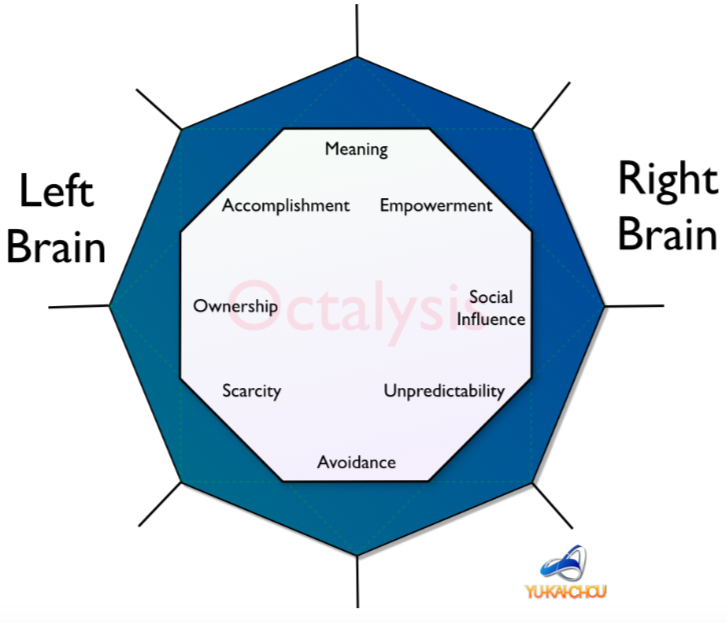
\includegraphics[keepaspectratio=true,scale=0.34]{figuras/brain.png}
	\caption{Divisão do octógono}
	Fonte: \cite{chou2017actionable}
	\label{octogono1}
\end{figure}

A estrutura do \textit{Octalysis} é organizada de forma que os núcleos relacionados à criatividade, auto expressão e dinâmica social são
representados dos lado direito do octógono ("\textit{Right Brain}"). Os núcleos relacionados à logica, pensamento analítico e propriedade são representados graficamente
no lado esquerdo (\textit{"Left Brain"}). É importante ressaltar que ``\textit{Right Brain}'' e \textit{``Left Brain''} não são literais no que se refere
à regiões do cérebro humano, a utilização destes termos é apenas um simbolismo.

\subsection{Gamificação \textit{White Hat} e \textit{Black Hat}}

Uma característica importante na representação dos núcleos motivacionais dentro do octógono é a forma como eles estão agrupados em relação ao impacto
que causam sobre os participantes. Os núcleos localizados na parte superior do octógono são considerados ``motivadores positivos'' enquanto os núcleos localizados
na parte inferior do octógono são considerados "motivadores negativos". Os \textit{cores} apresentados na parte superior são chamados de \textit{"White hat"} e os inferiores
são conhecidos como \textit{"Black hat"}. Na figura \ref{octogono} é apresentado a divisão dos núcleos levando em consideração o tipo de motivador em que cada um
é classificado.

\begin{figure}[h]
	\centering
	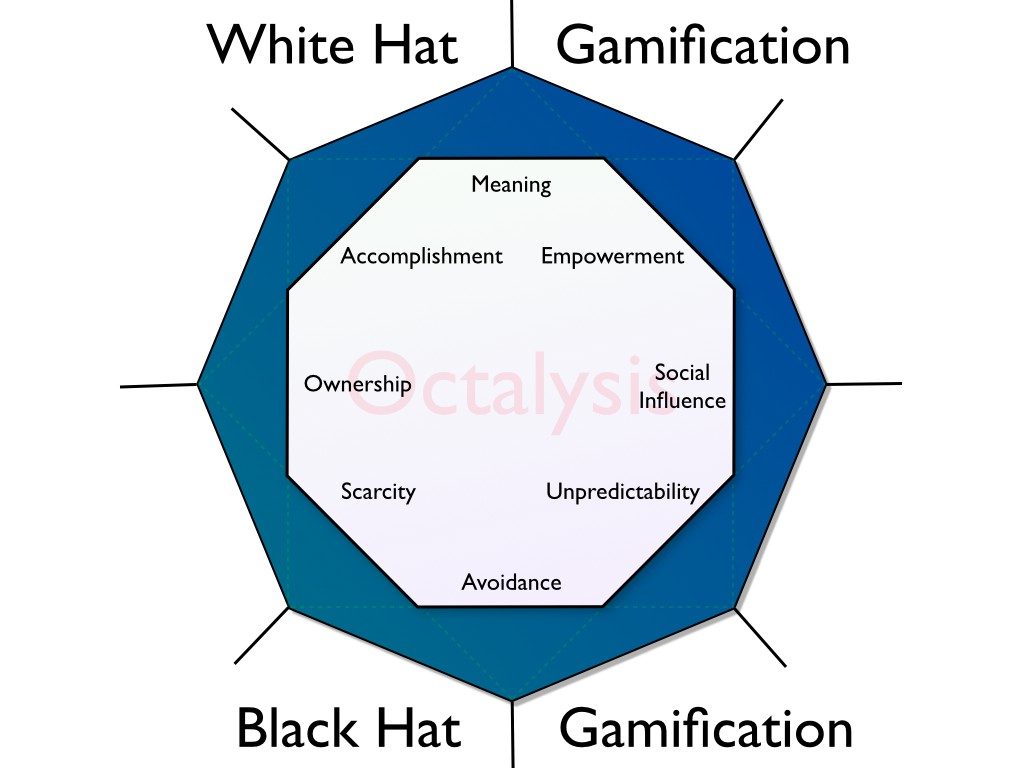
\includegraphics[keepaspectratio=true,scale=0.28]{figuras/octogono.jpg}
	\caption{Gamificação \textit{White hat} e \textit{Black hat}}
	Fonte: \cite{chou2017actionable}
	\label{octogono}
\end{figure}

\citeonline{chou2017actionable} apresenta um exemplo do que vem a ser os núcleos \textit{"White hat"} e \textit{"Black hat"}. Se algo é envolvente
por permitir que se expresse a criatividade, faz com que os indivíduos envolvidos se sintam bem sucedidos e poderosos, com certeza há um \textit{core} 
\textit{"White hat"} sendo utilizado. Por outro lado, se os envolvidos realizam determinadas ações por não saber o que acontecerá logo em seguida ou está
constantemente com medo que algo ruim possa acontecer, neste caso, há um \textit{core} \textit{"Black hat"} sendo utilizado.

Como apresentado por \citeonline{chou2017actionable}, não é porque alguma coisa é categorizada como \textit{"black"} que ela seja ruim. Se utilizadas
corretamente podem gerar resultados saudáveis e positivos. De acordo com \citeonline{chou2017actionable}, um profissional de gamificação deve sempre considerar
todos os \textit{core drive} objetivando obter resultados positivos e produtivos.


\subsection{Níveis \textit{Octalysis}}

O \textit{framework Octalysis} é dividido em vários níveis que, quanto mais alto forem, mais domínio por parte do ``gamificador'' é requerido \cite{chou2017actionable}.
Nas subseções que se seguem, são apresentadas as características relacionadas aos três primeiros níveis do \textit{octalysis}.

\subsubsection{Nível 1}
Para ser aplicado, este nível deve levar em consideração pontos fortes e fracos de vários produtos, este primeiro método permite identificar
que tipos de motivação são fracas para que se possa introduzir novas melhorias \cite{chou2017actionable}.

O segundo método consiste na criação de uma nova experiência baseada nos \textit{core drives} através de um processo sistemático.

Como citado em seções anteriores, neste nível sempre há a necessidade de se utilizar ao menos um \textit{core drive}, caso não seja utilizado nenhum
dos oito núcleos, a motivação é zero e nenhum progresso relativo à gamificação é alcançado \cite{chou2017actionable}.

\subsubsection{Nível 2}
Este nível envolve todas as quatro fases da jornada de um jogador. Em seguida são apresentadas cada uma das quatro fases, bem como suas características.

\begin{itemize}
	\item Descoberta: Experimentações e ganhos de experiências por parte dos jogadores;
	\item Entrada: Aprendizado das regras e ferramentas necessárias para jogar o \textit{game}.
	\item Dia a dia: Jornada regular de ações e comportamentos que os jogadores devem realizar para completar os objetivos;
	\item Fim de jogo: Manter os jogadores motivados a continuarem jogando.
	
\end{itemize}

\citeonline{chou2017actionable} argumenta que o motivo pelo qual as pessoas utilizam um produto no dia 1 muitas das vezes é bastante diferente do
motivo de uso no dia 100. Por este motivo, é importante se planejar cada uma das quatro fases envolvidas na trajetória dos jogadores. Caso não haja nenhum
\textit{core drive} envolvido em alguma das fases, o jogador não possui uma razão para passar para a próxima fase e ele simplesmente desiste.

\begin{figure}[h]
	\centering
	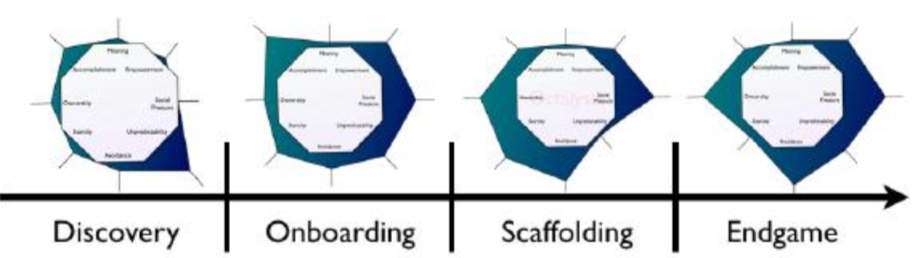
\includegraphics[keepaspectratio=true,scale=0.48]{figuras/fasesjornada.png}
	\caption{As fases da jornada de um jogador.}
	Fonte: \cite{chou2017actionable}
	\label{fasesjornada}
\end{figure}

Observando a figura \ref{fasesjornada}, é possível notar os \textit{core drives} mais proeminentes durante cada fase de experiência da jornada
dos jogadores.

\subsubsection{Nível 3}
Este nível está relacionado com a identificação dos perfis de jogadores e como eles se comportam quando estão envolvidos em jogos. Mesmo que seja
praticamente impossível, este nível permite aos projetistas de gamificação buscar atender as necessidades e motivações dos mais diferentes perfis.

\subsubsubsection{\textit{Design} de gamificação: Octalysis e Bartle}

Embora a classificação dos perfis dos jogadores seja uma proposta criada por \citeonline{bartle1996hearts}, \citeonline{chou2017actionable} apresenta um modelo
que une os perfis apresentados por Bartle com os \textit{core drives} apresentados no \textit{framework Octalysis} de forma a criar um \textit{design} de gamificação
mais apropriado para cada tipo de perfil.

Como apresentado por \citeonline{gamification} no livro ``Gamification: reinventando empresas a partir de jogos'' e com base nos estudos de \citeonline{bartle1996hearts}, 
existem quatro perfis de jogadores que possuem características e comportamentos específicos quando envolvidos em jogos. Cada um destes quatro perfis são apresentados na
subseção a seguir.

\subsubsection{Perfis de Jogadores} 

\subsubsubsection{Predadores (\textit{Killers})}
São aqueles jogadores que participam de uma competição pelo prazer de derrotar os adversários. O objetivo desse tipo de jogador é ser o melhor, não 
se importam com o que está em disputa. Possuem comportamentos agressivos e focados em conquistar a posição de liderança. Seus desejos de liderança se 
sobrepõem à cooperação.

\subsubsubsection{Realizadores (\textit{Achievers})}
A motivação destes jogadores consiste na realização de todas as atividades que o jogo apresenta. Esses jogadores apreciam a sensação constante
de vitória mesmo que os objetivos a serem alcançados não sejam tão relevantes ou significativos. Atuam de maneira cordialmente competitiva, mesmo que não estejam
liderando algum placar. São caracterizados por se destacarem dos demais jogadores de maneira leal, isto é, por meio de suas próprias conquistas.

\subsubsubsection{Exploradores (\textit{Explorers})}
Este é um grupo que se caracteriza pela busca e interesse em desvendar todas as possibilidades dos jogos. São indivíduos curiosos que se dedicam em estudar
e desenvolver habilidade que lhes permitam solucionar os mais diversos desafios. Para este tipo de perfil, a trejetória é mais importante que a conquista.

\subsubsubsection{Socializadores (\textit{Socializers})}
São, no geral, os indivíduos que enxergam o contato com jogos como um meio de interação social. Mais significativo que atingir os objetivos propostos ou
realizar derterminadas tarefas é a oportunidade de reforçar e estabelecer vínculos sociais. Os socializadores, em sua maioria, preferem jogos cooperativos
que necessitam de trabalho conjunto. Estes representam 80\% do total de jogadores.

\subsubsection{Relação entre \textit{Core drives} e Perfis de jogadores}
Como apresentado por \citeonline{chou2017actionable} em seu livro \textit{"Actionable Gamification – Beyond Points, Badges, and Leaderboards"}, para cada perfil de jogador,
exitem um conjunto de \textit{core drives} que os motivam  a engajarem no desenvolvimento e realização de determinadas ações dentro de um jogo. Na tabela a seguir ,
são apresentados os \textit{core drives} predominantes em cada perfil que, se utilizados de maneira correta, podem aumentar o interesse e engajamento dos perfis identificados na seção anterior.


\begin{table}[h]
	\centering
	\resizebox{\textwidth}{!}{%
	\begin{tabular}{|p{3cm}|p{3cm}|p{3cm}|p{3cm}|p{3cm}|p{3cm}|p{3cm}|p{3cm}|p{3cm}|}
	\hline
	\textbf{Perfil} & \textbf{CD 1 - Significado épico e chamado} & \textbf{CD 2 - Desenvolvimento e Conquista} & \textbf{CD 3 - Empoderamento e feedback} & \textbf{CD 4 - Propriedade e posse}  & \textbf{CD 5 - Influência e relacionamento social } & \textbf{CD 6 - Escassez e impaciência} & \textbf{CD 7 - Imprevisibilidade e curiosidade} & \textbf{CD 8 - Prevenção e perda}  \\ \hline
	Predadores (\textit{Killers}) & & x &  &  & x & & &    \\ \hline
	Realizadores (\textit{Achievers}) & & x & &  & & x & & \\ \hline
	Exploradores (\textit{Explorers}) & &  &  & & &  & x & \\ \hline
	Socializadores (\textit{Socializers}) & & &  &  & x & &  & \\ \hline
	\end{tabular}%
	}
	\caption{Principais \textit{core drives} envolvidos em cada perfil de jogador}
	\label{perfil}
	Fonte: \cite{chou2017actionable}
	% \small{Quadro 1 - Classificação das questões, \citeonline{raposo2016desafio}} 
\end{table}

\pagebreak

\citeonline{chou2017actionable} apresenta um gráfico relacionando os quatro perfis dos jogadores com os \textit{core drives} característicos
de cada um deles. O gráfico é apresentado na figura \ref{perfiljogadores}.

\begin{figure}[h]
	\centering
	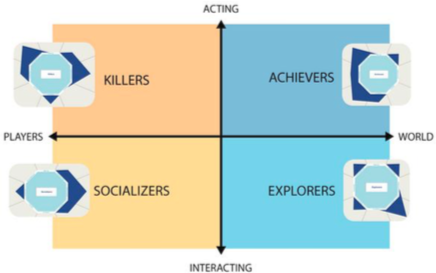
\includegraphics[keepaspectratio=true,scale=0.6]{figuras/perfiljogadores.png}
	\caption{Perfil de jogadores}
	Fonte: \cite{chou2017actionable}
	\label{perfiljogadores}
\end{figure}
 
Na figura \ref{nivel3}, são apresentados os \textit{core drives} mais utilizados em cada uma das quatro fases da jornada dos jogadores levando em
consideração os quatro tipos de perfis identificados por \citeonline{bartle1996hearts}.

\begin{figure}[h]
	\centering
	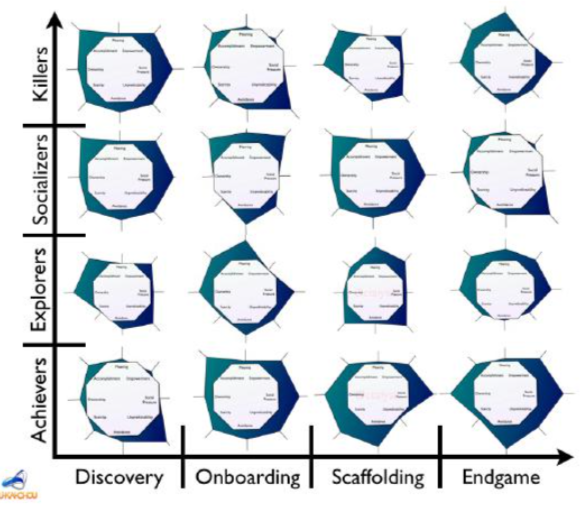
\includegraphics[keepaspectratio=true,scale=0.5]{figuras/nivel3.png}
	\caption{\textit{Core drives} mais utilizados de acordo com as fases e perfis de jogadores.}
	Fonte: \cite{chou2017actionable}
	\label{nivel3}
\end{figure}

\section{Modelagem de banco de dados}

Existem diversas formas de se representar graficamente a forma como uma base de dados deverá estar consolidada em um banco de
dados após sua implementação. Nesta seção, apresenta-se uma forma específica de modelagem de base de dados, bem como suas características.

\subsection{Diagrama entidade-relacionamento}
Segundo \citeonline{projetobancodedados} , a abordagem mais utilizada e conhecida é a 
entidade-relacionamento (ER) onde o modelo de dados é geralmente representado graficamente através
de um diagrama entidade-relacionamento (DER). Esta abordagem foi criada em 1976 por Peter Chen e
é considerada como um padrão para a modelagem conceitual.

A abordagem entidade-relacionamento é baseada em dois principais pilares que são apresentados em seguida.

\subsubsection{Entidade}
De acordo com \citeonline{projetobancodedados}, uma entidade, no modelo conceitual, representa um conjunto
de objetos da realidade modelada. Seu principal objetivo é modelar de forma abstrata um banco de dados, onde
se te interesse somente nos objetos sobre os quais deseja-se manter informações. No DER, uma entidade é representada
por meio de um retângulo contendo o nome da entidade.
 
\subsubsection{Relacionamento}
Como apresentado por \citeonline{projetobancodedados}, o DER permite a especificar as propriedades dos objetos
que serão armazenados no banco de dados, como por exemplo o relacionamento/associação entre os objetos. No DER,
um relacionamento é representado por meio de um losango que são ligados por linhas aos retângulos que representam
as entidades que participam de um determinado relacionamento.

Na figura \ref{figura1} é apresentado um exemplo simples de um diagrama entidade-relacionamento (DER). É possível notar 
no diagrama a existência de atributos e cardinalidade, estes dois são apresentados logo em seguida.

\begin{figure}[h]
	\centering
	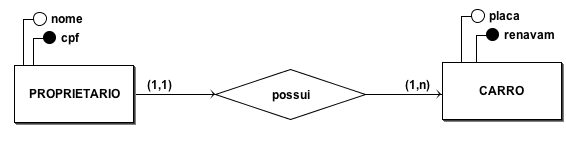
\includegraphics[keepaspectratio=true,scale=0.5]{figuras/figura1.png}
	\caption{Exemplo de DER}
	Fonte: Autor
	\label{figura1}
\end{figure}

Os atributos correspondem às características/qualidades que descrevem uma entidade, são representados por
elipses ou círculos acompanhados por seus respectivos nomes \cite{sistemadebancos}.

As cardinalidades representam a restrição do número de objetos que podem participar do relacionamento. Na notação
de Peter Chen, as cardinalidade são apresentadas próximas às ligações de relacionamento e são compostas da quantidade
mínima e máxima de objetos que podem participar do relacionamento. Tais características podem ser vistas 
na figura \ref{figura1} \cite{sistemadebancos}.

\subsection{Diagrama Lógico}
O diagrama lógico leva em consideração as limitações e implementa recursos como adequação de padrão e nomenclatura, define as
chaves primárias e estrangeiras, normalização, integridade referencial, entre outras. Para o modelo lógico deve ser criado 
levando em conta os exemplos de modelagem de dados criados no modelo conceitual \cite{sistemadebancos}.


% Na figura \ref{figura2} é apresentado um exemplo simples de um diagrama lógico (DL). É possível notar 
% no diagrama a existência dos atributos, seus tipos (tipos de dados), chaves entre outras características necessária para o correto
% desenvolvimento da base de dados.

% \begin{figure}[h]
% 	\centering
% 	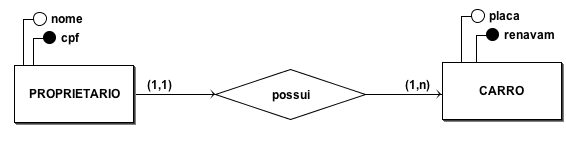
\includegraphics[keepaspectratio=true,scale=0.5]{figuras/figura1.png}
% 	\caption{Exemplo de DER}
% 	Fonte: Autor
% 	\label{figura2}
% \end{figure}
\section{Metodologia cascata}

De acordo com \citeonline{semedo2012ganhos}, metodologia pode ser definida como um conjunto de procedimentos, técnicas, documentação e ferramentas que 
auxiliam os responsáveis ou interessados no desenvolvimento e implementação de um sistema de informação. Na maioria das vezes, o sucesso
de um projeto de software depende de vários fatores que vão desde o planejamento à escolha mais adequada de uma metodologia.

O modelo cascata, também conhecido como modelo tradicional, é uma das metodologias mais antigas e conhecidas. A utilização desta 
metodologia consiste em seguir o desenvolvimento do projeto de forma sequencial, onde só se deve passar para os níveis seguintes após
a conclusão do nível anterior. Esta metodologia envolve duas grandes fases: levantamento de requisitos/necessidades e design. \cite{semedo2012ganhos}

Muitos autores desencorajam a utilização da metodologia cascata no desenvolvimento de grandes sistemas, como é o caso do pesquisador
\apudonline{gilb1988principles}{semedo2012ganhos}  e \apudonline{brooks}{semedo2012ganhos}. Este tipo de metodologia deve ser usada apenas em situações onde os requisitos do software são estáveis e requisitos
que possam vir a surgir no futuro sejam previsíveis. \cite{semedo2012ganhos}


No modelo cascata apresentado por \citeonline{pressman} no livro "Engenharia de Software: Uma abordagem profissional", o autor
apresenta cinco fases sequenciais que devem ser satisfeitas no desenvolvimento de um sistema obedecendo esta metodologia(cascata). 
Cada uma das cinco fases podem ser vistas na figura \ref{cascata} apresentada logo em seguida.

\begin{figure}[h]
	\centering
	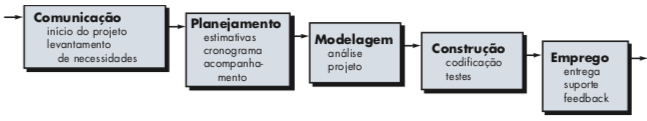
\includegraphics[keepaspectratio=true,scale=0.6]{figuras/cascata.png}
	\caption{Modelo cascata}
	Fonte: \cite{pressman}
	\label{cascata}
\end{figure}


\chapter{Metodologia}

Neste capítulo, são apresentados com detalhes o passo a passo realizado para a construção de uma ferramenta web de apoio ao ensino e aprendizagem 
de programação gamificada.

\section{\textit{Core drives}}

	Os \textit{core drives} implementados no desenvolvimento da aplicação, foram definidos a partir de um questionário que teve como objetivo identificar as características 
em jogos que mais atraem os alunos/jogadores.

	A partir de análises realizadas no conjunto de dados obtidos, identificou-se predominantemente os \textit{core drives} apresentados na tabela \ref{core}.

	\begin{table}[h]
		\centering
		\resizebox{.9\textwidth}{!}{%
		\begin{tabular}{|p{7cm}|p{7cm}|}
		\hline
		\textbf{\textit{Core drive}} & \textbf{Técnicas} \\ \hline
		Desenvolvimento e conquista & Pontos, \textit{ranking}, lista de desafios e barra de progresso.  \\ \hline
		Empoderamento e \textit{feedback} & Desbloqueio de marcos, \textit{boost} e \textit{feedback} \\ \hline
		Significado épico e chamado &  Narrativa e elitismo\\ \hline
		Prevenção e perda & Perda de pontos e perda de progresso \\ \hline
		\end{tabular}%
		}
		\caption{\textit{Core drives} implementados}
		\label{core}
		Fonte: Autor
		% \small{Quadro 1 - Classificação das questões, \citeonline{raposo2016desafio}} 
	\end{table}

\subsection{Desenvolvimento e conquista}
\subsubsection{Pontos}
	A medida que os alunos/jogadores realizam alguma entre a variedade de atividades disponíveis na ferramenta, o mesmo adquire pontos.
As atividades possuem diferentes pontuações de acordo com sua natureza e dificuldade. Na tabela \ref{pontos}, são apresentados as atividades e suas
respectivas pontuações.

\begin{table}[h]
	\centering
	\resizebox{.9\textwidth}{!}{%
	\begin{tabular}{|p{7cm}|p{3cm}|}
	\hline
	\textbf{Atividade} & \textbf{Pontuação} \\ \hline
	Questões Quiz & 10  \\ \hline
	Desafios (jogador vs PC) & 100\\ \hline
	Criar um desafio para outtro jogador (jogador vs jogador) &  100\\ \hline
	Responder desafios de outros jogadores (jogador vs jogador) &  100\\ \hline
	Avaliar resposta do desafiado (jogador vs jogador) & 100 \\ \hline
	\end{tabular}%
	}
	\caption{Pontuações}
	\label{pontos}
	Fonte: Autor
	% \small{Quadro 1 - Classificação das questões, \citeonline{raposo2016desafio}} 
\end{table}
\pagebreak 

\subsubsection{\textit{Ranking}}
	A ferramenta fornece uma página dedicada à apresentar as pontuações dos jogadores bem como seus nomes, matrículas e posições, desta forma, todos os jogadores/alunos
 têm a noção do seu progresso em relação aos demais usuários do sistema. Tornando, desta forma, a busca por pontuações e usp dos módulos disponíveis mais competitivos.

\subsubsection{Lista de desafios}
	O sistema possui um módulo destinado inteiramente para desafios que podem ser cadastrados pelo administrador do sistema ou em casos de desafios jogador vs jogador, os próprios
 usuários da ferramenta podem criar seus próprios desafios.

\subsubsection{Barra de progresso}

	A ferramenta possui uma página de perfil contendo diversas informações do jogador, isso inclui uma barra de progresso que mostra a evolução do jogador na utilização da
 ferramenta e seu avanço nos doze níveis disponíveis na mesma.

 \subsection{Empoderamento e \textit{feedback}}
	 \subsubsection{Desbloqueio de marcos}
	A ferramenta possui um sistema de divisão de conteúdos por níveis. No total existem 12 níveis que vão sendo desbloqueados a medida que os jogadores conquistam determinadas pontuações.

	Na tabela \ref{pontos} são apresentadas as pontuações necessárias para desbloquear cada nível.


\begin{table}[h]
	\centering
	\resizebox{.9\textwidth}{!}{%
	\begin{tabular}{|p{7cm}|p{3cm}|}
	\hline
	\textbf{Nível} & \textbf{Pontuação} \\ \hline
	1 & < 800  \\ \hline
	2 & > 800\\ \hline
	3 & > 1600 \\ \hline
	4 & > 3200\\ \hline
	5 & > 6400 \\ \hline
	6 & > 12800  \\ \hline
	7 & > 25600\\ \hline
	8 & > 51200\\ \hline
	9 & > 102400\\ \hline
	10 & > 204800 \\ \hline
	11 & > 409600  \\ \hline
	12 & > 819200\\ \hline
	\end{tabular}%
	}
	\caption{Pontuações}
	\label{pontos}
	Fonte: Autor
	% \small{Quadro 1 - Classificação das questões, \citeonline{raposo2016desafio}} 
\end{table}

\subsubsection{\textit{Feedback}}

A ferramenta conta com diversos mecanismo de \textit{feedbacks}, que estão presentes em todos os módulos disponíveis.
Os \textit{feedbacks} seguem a temática da ferramenta, ou seja, animações com temática Orc. Este mecanismo de \textit{feedback} ocorre, por exemplo, quando um jogador progride nos níveis
, responde um desafiou, elabora um novo desafio, realiza ataques, entre outros.

Em geral, as animações e \textit{feedbacks} buscam encorajar os jogadores a realizarem ações que faça com que o mesmo tenha maior engajamento no uso
da ferramenta.

\subsubsubsection{\textit{Booster}}
A ferramenta implementa um sistema de \textit{booster} que permite ao jogador ter seus pontos multiplicados
de acordo com o número de acertos que o mesmo obtiver e dependendo do tipo de \textit{booster} utilizado.

Os ítens de \textit{booster} são representados pelas espadas no módulo "loja", os custos para sua obtenção 
e fator multiplicativo podem ser vistos na figura \ref{espadas}

\begin{figure}[h]
	\centering
	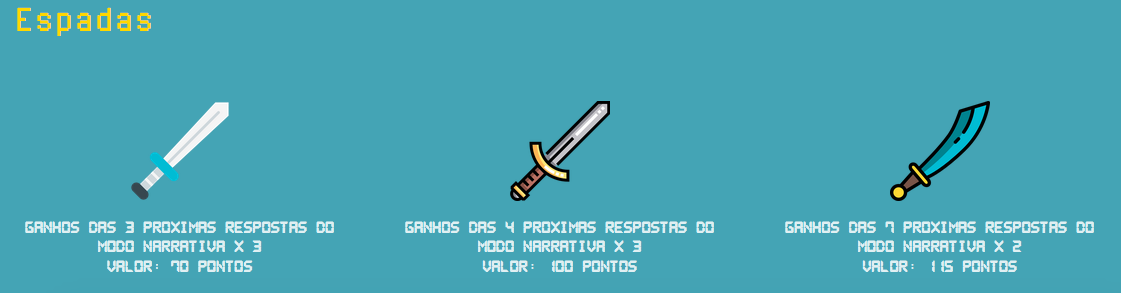
\includegraphics[keepaspectratio=true,scale=0.4]{figuras/espadas.png}
	\caption{Tipos de \textit{booster}.}
	Fonte: Autor
	\label{espadas}
\end{figure}

\subsection{Significado épico e chamado}
\subsubsection{Elitismo}
A ferramenta visa valorizar seus participantes de forma a enaltecer sua importância no contexto da história 
elaborada. Isto é, o jogador é peça fundamental na ferramenta, ele é o responsável por salvar sua aldeia e povo
da invasão, que somente pode ser feito por ele.


\subsubsection{Narrativa}
A aplicação possui uma narrativa que elaborado especialmente objetivando envolver o jogador/aluno
em uma temática Orc. Basicamente, ao iniciar o primeiro acesso na aplicação, o jogador é apresentado brevemente à história temática onde,
por meio de uma voz gravada e processada, é apresentado todo o contexto da jornada que o mesmo deverá seguir.

Após a apresentação da jornada e temática da aplicação, São presentado seis personagens com distintas características onde, o aluno deve escolher o personagem
que lhe mais atrair, seja pela história do personagem ou características como: poderes, trajes e etc.

\subsection{Prevenção e perda}
\subsubsection{Perda de pontos}
Na ferramenta, existe um painel que permitem aos jogadores elaborar estratégias mais dinâmicas. Uma das formas de se obter vantagem estratégica na aplicação, é atacar
outros jogadores diretamente ou todos os jogadores de um vez só, existem diversos ítens como porções e etc, que causam perda de pontos
dos jogadores alvos. As porções, valor do dano, valor de uso(custo) e etc, são apresentados nas figuras \ref{porcoes} e \ref{porcoes2}

\begin{figure}[h]
	\centering
	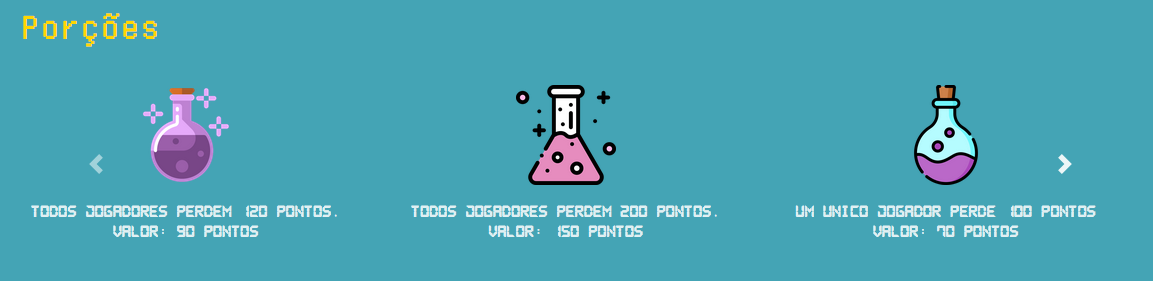
\includegraphics[keepaspectratio=true,scale=0.4]{figuras/p1.png}
	\caption{Tipos de porções.}
	Fonte: Autor
	\label{porcoes}
\end{figure}

\begin{figure}[h]
	\centering
	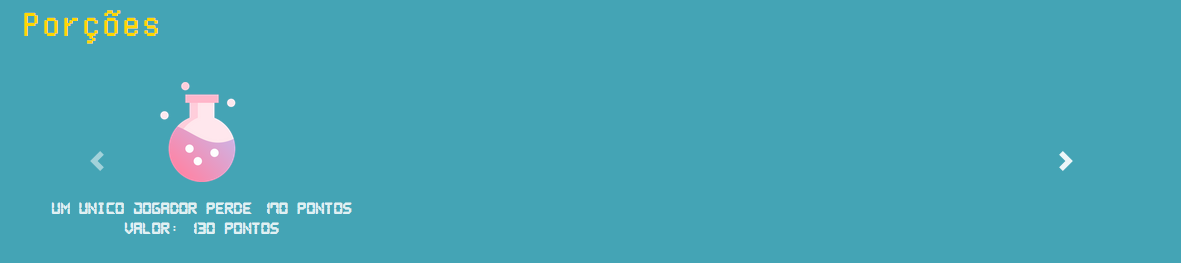
\includegraphics[keepaspectratio=true,scale=0.4]{figuras/p2.png}
	\caption{Tipos de porções.}
	Fonte: Autor
	\label{porcoes2}
\end{figure}

\subsubsection{Perda de progresso}
Com a conquista de determinadas pontuações, novos \textit{levels} vão sendo liberados. O contrário também ocorre, ou seja, ao perder 
pontos e se a pontuação restante for menor que o necessário para o \textit{level} ser desbloqueado, o jogador é 
automáticamente rebaixado para o nível que sua pontuação for compatível.

Isso implica, por exemplo, ma necessidade de o jogador ter que estudar e refazer questões, desafios entre outras atividades que 
ele já havia solucionado.

\section{Requisitos}

Tendo como base a pesquisa realizada na primeira parte deste trabalho, nesta seção, são apresentados os requisitos implementados na construção da 
ferramenta.

Como apresentado no referencial teórico deste trabalho, o \textit{framework octalysis} é dividido em vários níveis. Neste trabalho, a solução tecnológica
foi construída sobre o nível 1.

Na tabela a seguir, é apresentado uma comparação entre os requsitos levantados em relação aos implementados.

\begin{table}[h]
	\centering
	\resizebox{.9\textwidth}{!}{%
	\begin{tabular}{|l|l|l|l|}
	\hline
	\textbf{Identificador} & \textbf{Requisito} & \textbf{Implementado?}\\ \hline
	RF 01 & CRUD de jogadores & Sim \\ \hline
	RF 02 & Ativar/desativar perfil de jogadores & Sim \\ \hline
	RF 03 & Rankeamento de jogadores & Sim\\ \hline
	RF 04 & CRUD de disciplinas & Não\\ \hline
	RF 05 & CRUD de turmas & Não\\ \hline
	RF 06 & CRUD de conteúdos para estudo & Sim\\ \hline
	RF 07 & CRUD de desafios & Sim\\ \hline
	RF 08 & Sistema de recompensas (pontuação) & Sim\\ \hline
	RF 09 & Dashboard pessoal de desempenho (jogadores) & Sim \\ \hline
	RF 10 & CRUD de professores de disciplinas & Não\\ \hline
	RF 11 & Painel de acompanhamento de desempenho dos alunos (professores) & Não \\ \hline
	RF 12 & Narrativa temática & Sim\\ \hline
	RF 13 & Personagens e guerreiros da narrativa & Sim\\ \hline
	RF 14 & Lógica de progressão de jogadores (\textit{levels}) & Sim\\ \hline
	RF 15 & CRUD de linguagens de programação & Sim \\ \hline
	RF 16 & Desafios entre jogadores (individual) & Sim\\ \hline
	RF 17 & CRUD de questões & Sim\\ \hline
	RF 18 & Desafios entre times/grupos & Não\\ \hline
	RF 19 & Torneios/campeonatos entre turmas & Não \\ \hline
	\end{tabular}%
	}
	\caption{Requisitos implementados}
	Fonte: {Autor}
	% \small{Quadro 2 - Requisitos funcionais} 
\end{table}


\chapter{Solução proposta}

\section{Ferramentas de desenvolvimento}
A escolha das ferramentas de desenvolvimento e demais tecnologias, foram realizadas com base em experiências prévias, disponibilidade de documentações e comunidades de apoio ao desenvolvedor.

A seguir são apresentadas as principais tecnologias utilizadas no desenvolvimento da ferramenta bem como uma breve descrição de suas características.

\subsection{\textit{Backend}}

\begin{itemize}
	\item Java: Linguagem de programação orientada a objetos desenvolvida na década de 90.Diferente das linguagens de programação
		modernas que são compiladas para código nativo, a linguagem java é compilada para um \textit{bytecode} que é interpretado por uma máquina
		virtual (\textit{java virtual machine}). Por conta disso, a linguagem torna-se altamente portável, isto é, independente de plataforma \cite{java}.
	\item MySql: Sistema de gerenciamento de banco de dados que utiliza linguagem sql como interface. Voltado para o armazenamento e manutenção 
		de registros de um banco de dados \cite{mysql}.
	\item Maven: Ferramenta de automação de compilação muito utilizada em projetos que envolvem a linguagem java. O maven
		utiliza um arquivo \textit{xml} (POM) para descrever o projeto de software sendo implementado, suas dependências, componentes
		externos, \textit{plugins} necessários, diretórios e ordem de compilação \cite{maven}.
	\item Jersey: \textit{Framework} que facilita o desenvolvimento de APIs (Application Programming Interface) RESTful \cite{jersey}.
	\item JDBC: \textit{Driver} que possui um conjunto de classes e interfaces java que permitem o envio/comunicação com qualquer
		banco de dados relacional. Permitindo interligar a aplicação com um banco de dados \cite{jdbc}.
	\item Tomcat: Consiste em um servidor de aplicações java que permite que o mesmo funcione na \textit{web} \cite{tomcat}.

\end{itemize}

\subsection{\textit{Frontend}}
\begin{itemize}
	\item Vue.js: \textit{Framework} javaScript voltado para o desenvolvimento de interfaces de usuário \cite{vue}.
	\item Axios: É um cliente HTTP que permite consumir e exibir dados de uma API (Application Programming Interface) de forma facilitada e ágil \cite{axios}.
	\item Html: Linguagem de marcação bastante utilizada na construção de páginas web. Que podem ser interpretados por 
		qualquer navegador \cite{html}.
	\item CSS: Mecanismo que permite adicionar cores, fontes, espaçamentos e efeitos em um documento \textit{web} (html). \cite{css}
	\item Bootstrap:\textit{Framework web} voltado para o desenvolvimento de interfaces para aplicações e sites usando HTML, CSS e JavaScript, melhorando
		a experiência do usuário, tornando um site amigável e responsível \cite{bootstrap}.
	\item Json: \textit{JavaScript Object Notation} é uma formatação de troca de dados. Possui formato textual e é completamente independente de linguagem. É
		consituido por conjuntos de chave e seu respectivo valor \cite{json}.
\end{itemize}

\section{Segurança dos dados}
Visando prover maior segurança das informações dos jogadores/usuários, informações críticas como senhas de usuários,
são persistidas no banco de dados de forma criptografada. Desta forma, nem os desenvolvedores/manetedores ou possíveis 
tentativas de ataque \textit{hacker} têm acesso a essa informação.

Nessa solução, utilizou-se como algoritmo de criptografia o MD5.

\section{Arquitetura}

No desenvolvimento da ferramenta, utilizou-se o "n camadas". Esse tipo
de arquitetura consiste na separação de responsabilidades específicas para cada uma das camadas presentes 
na construção do sistema \cite{MSF}. A letra ``n'' representa a quantidade de camadas em que a construção do sistema 
está dividida, nesta solução, o desenvolvimento do sistema está dividido em 4 camadas que são: apresentação, serviço, modelo
e armazenamento.

O modelo simplificado apresentado na figura \ref{arquitetura} demonstra como ocorre o fluxo de comunicação entre as principais tecnologias
usadas no desenvolvimento.

\begin{figure}[h]
	\centering
	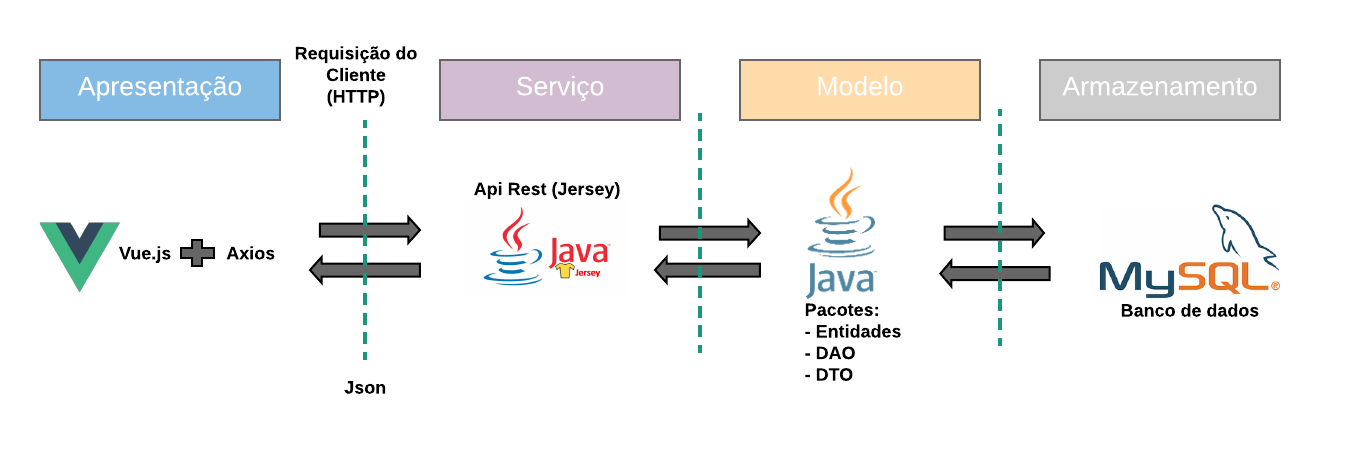
\includegraphics[keepaspectratio=true,scale=0.8]{figuras/arquitetura.png}
	\caption{Representação da arquitetura do sistema.}
	Fonte: {Autor}
	\label{arquitetura}
\end{figure}	

\subsection{Camada 1: Apresentação}
Esta camada envolve todas as tecnologias responsáveis pela apresentação de informações ao usuário e realização de requisições para obter as informações
a serem apresentadas. As principais tecnologias utilizadas para a consolidação desta camada foram: HTML, CSS, Vue.js, Axios (requisições) e bootstrap.

\subsection{Camada 2: Serviço}
A camada de serviço é responsável pelo preparo e disponibilização de informações obedecendo uma certa estrutura (json para esta solução) quando estas forem requisitadas. 
Cabe a ela iniciar a comunicação com as subcamadas de forma a solicitar que determinadas informações sejam recuperadas e organizar estas informações em uma estrutura que seja compatível
com o formato de troca de dados estabelecido. Para a construção do serviço, utilizou-se o \textit{framework} de construção de APIs REST, Jersey.

\subsection{Camada 3: Modelo}
Nesta camada são organizados em pacotes todos os arquivos necessários para realizar o mapeamento de objetos para os tipos de dados aceitos pelo banco de dados
adotado e obter uma conexão com o banco de dados. Esses dois itens citados são feitas por classes DAO (Objeto de Acesso a Dados).

Além das responsabilidades citadas no parágrafo anterior, cabe a esta camada a responsabilidade de definir a estrutura de transferência de dados entre os subsistemas
do software. Este padrão é conhecido como DTO (Objeto de Transferência de Dados) e geralmente são utilizados em conjunto com objetos de negócio de forma a se obter maior
flexibilidade no acesso a determinados dados.

\subsection{Camada 4: Armazenamento}
Esta camada consiste na utilização de um sistema gerenciador de banco de dados (SGBD), mySql para esta solução, que passa a ser responsável pelo armazenamento de forma segura e consistente
dos dados do sistema. Além de realizar o armazenamento, o SGBD é responsável por recuperar e manipular informações sempre que for necessário e fornece-las sempre que forem solicitadas.

\section{Desenvolvimento cascata}

No desenvolvimento da ferramenta, escolheu-se a metodologia cascata devido a natureza de desenvolvimento deste trabalho ser compatível com as 
catacterísticas propostas pela metodologia. O desenvolvimento da ferramenta partiu da definição dos requisitos, planejamento, desenvolvimento, testes e entrega final.

As características desta metodologia podem ser apreciadas em detalhes no referencial teórico deste trabalho.

\begin{figure}[h]
	\centering
	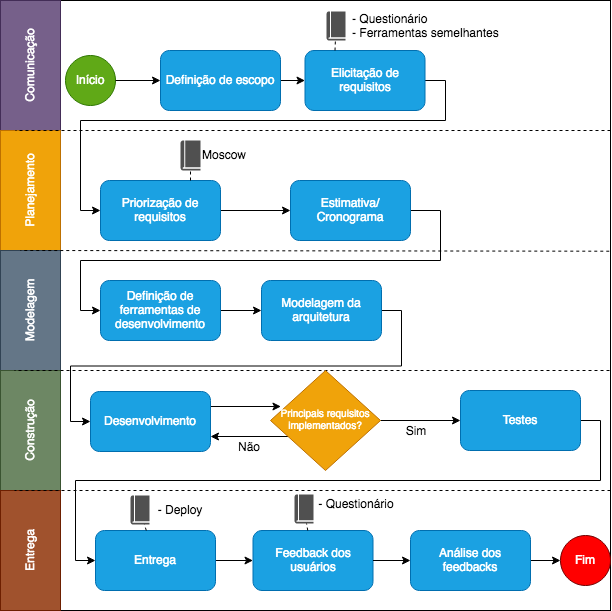
\includegraphics[keepaspectratio=true,scale=0.6]{figuras/modeloprocesso.png}
	\caption{Modelo de processos com principais atividades}
	Fonte: {Autor}
	\label{modeloprocesso}
\end{figure}	

No modelo apresentado na figura \ref{modeloprocesso}, é possível identificar em cada fase as principais atividades, iniciando pela definição
do escopo do projeto, elicitação de requisitos por meio da aplicação de um questionário e extração de algumas características
de \textit{design} de outras ferramentas e jogos, priorização dos requisitos por meio da ferramenta \textit{moscow},
definição das tecnologias de desenvolvimento utilizadas, modelagem arquitetural da ferramenta construída, desenvolvimento da ferramenta utilizando ferramentas e
 seguindo metodologia definida, testes, disponibilização da versão a ser utilizada como foco 
de análise, coleta de \textit{feedback} por meio da aplicação de questionário e análise dos dados.  

\section{Hospedagem}
Após a conclusão da construção da ferramenta, iniciou-se um estudo em cima de serviços de hospedagem.
Nesta fase também foi levado em consideração, assim como todas as tecnologias utilizadas no desenvolvimento desta ferramenta, os conhecimentos prévios e experiências com o serviço.

Com relação ao banco de dados, utilizou-se o próprio heroku como hospedagem. Embora aplicação e o banco de dados estejam hospedados neste serviço, os dois são independentes um do outro, isto é,Em caso de indisponibilidade de um destes, 
o outro não é afetado no que se refere a disponibilidade do serviço.
\pagebreak

\section{Modelagem de dados}
Como apresentado no referencial teórico de trabalho, existem diversas formas de representar em forma de diagrama banco de dados. Neste trabalho utilizou-se a diagramação de Peter Chen.
\begin{figure}[h]
	\centering
	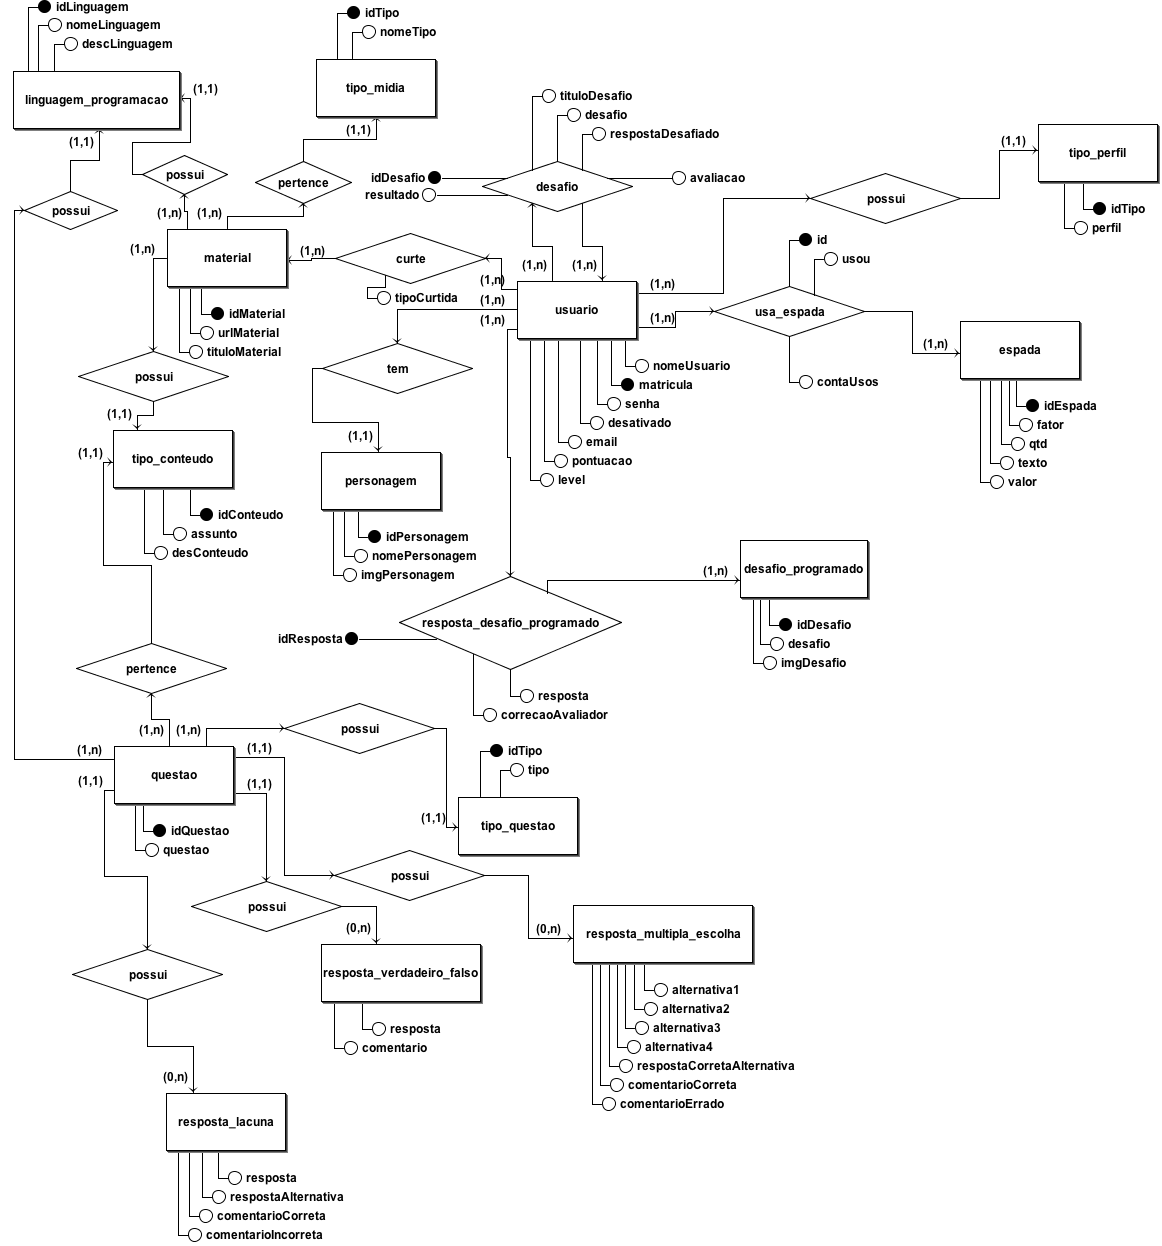
\includegraphics[keepaspectratio=true,scale=0.4]{figuras/der.png}
	\caption{DER da ferramenta}
	Fonte: Autor
	\label{figura2}
\end{figure}
\pagebreak

\begin{figure}[h]
	\centering
	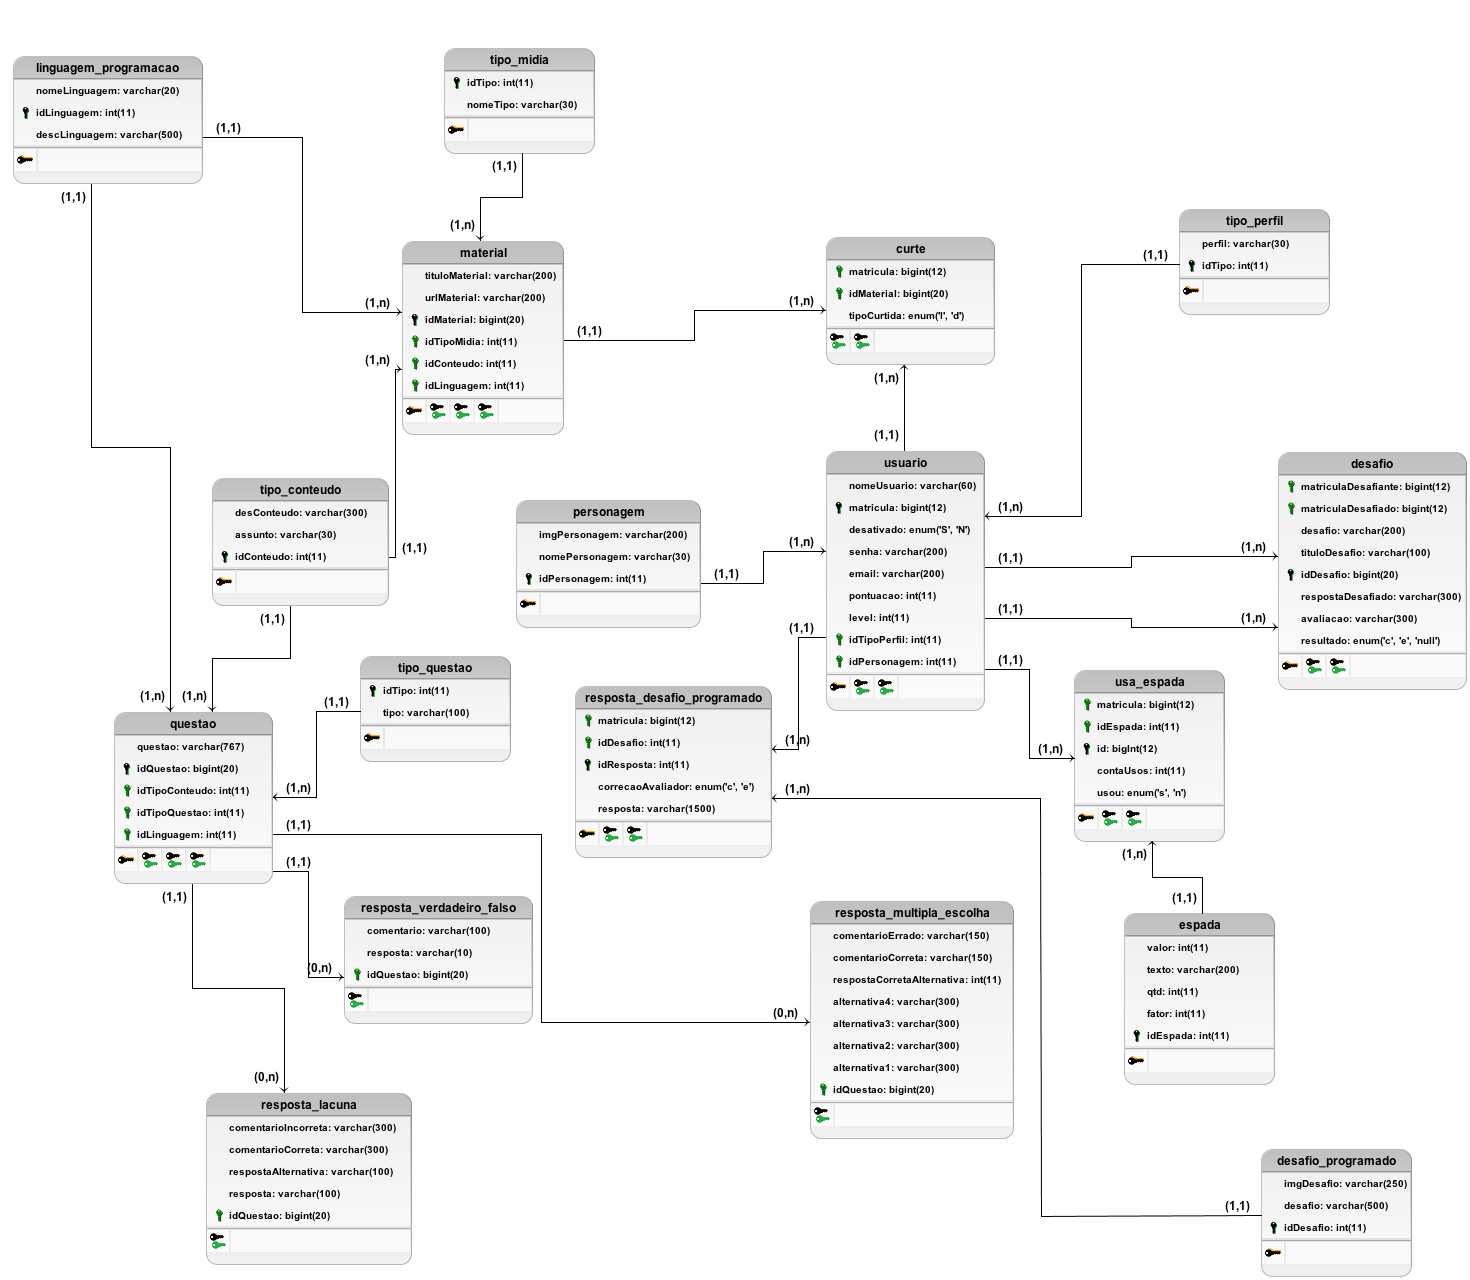
\includegraphics[keepaspectratio=true,scale=0.32]{figuras/dl.png}
	\caption{DL da ferramenta}
	Fonte: Autor
	\label{figura3}
\end{figure}

\section{Características específicas da ferramenta}

Nesta seção, são apresentados os elementos característicos da ferramenta como: personagens, narrativa, temática entre outros 
elementos que foram pensados como forma de gamificar as atividades de aprendizagem de programação.

\subsection{Narrativa}

Com o objetivo de aumentar o engajamento dos estudantes/jogadores, fora desenvolvida uma história que se passa em um mundo 
onde criaturas (Orcs) invadem o vilarejo do jogador que, motivado pelo desejo de vingança e tendo sido escolhido entre uma legião 
de outros guerreiro, dá início à jornada onde o mesmo deve cumprir com desafios como: quiz, desafiar outros jogadores entre outras
atividades que dão ao jogador pontos que podem ser trocados por itens ou serem acumulados afim de obter boas posições nos \textit{rankings}.

\subsection{Personagens}

Ao jogador, após a realização do primeiro \textit{login} na ferramenta, são apresentados seis personagens com diferentes características, onde o jogador
deve selecionar um único personagem para iniciar a jornada de aprendizado. Ao selecionar um determinado personagem, não é permitido ao jogador/estudante 
modifica-lo no decorrer do uso da ferramenta.

Os personagens são apresentados a seguir.

\subsubsection{Aisha}
\begin{figure}[h]
	\centering
	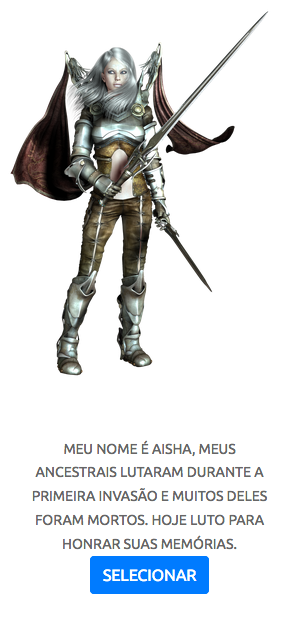
\includegraphics[keepaspectratio=true,scale=0.6]{figuras/aisha.png}
	\caption{Personagem Aisha}
	Fonte: Autor
	\label{aisha}
\end{figure}

\clearpage

\subsubsection{Voxter}
\begin{figure}[h]
	\centering
	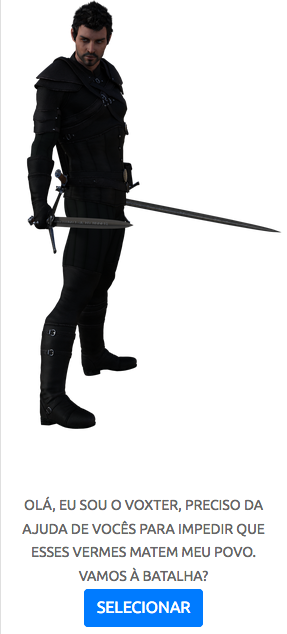
\includegraphics[keepaspectratio=true,scale=0.6]{figuras/voxter.png}
	\caption{Personagem Voxter}
	Fonte: Autor
	\label{voxter}
\end{figure}
\clearpage
\subsubsection{Lince}
\begin{figure}[h]
	\centering
	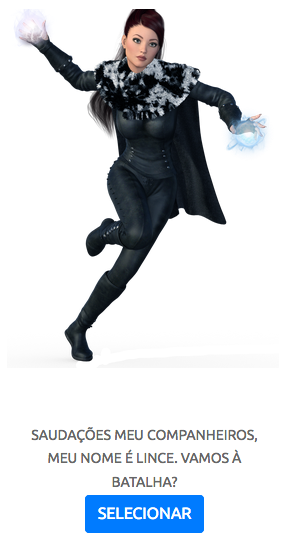
\includegraphics[keepaspectratio=true,scale=0.6]{figuras/lince.png}
	\caption{Personagem Lince}
	Fonte: Autor
	\label{lince}
\end{figure}
\clearpage
\subsubsection{Amazona}
\begin{figure}[h]
	\centering
	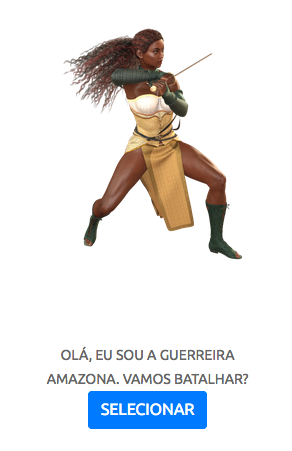
\includegraphics[keepaspectratio=true,scale=0.6]{figuras/amazona.png}
	\caption{Personagem Amazona}
	Fonte: Autor
	\label{amazona}
\end{figure}
\clearpage
\subsubsection{Tymer}
\begin{figure}[h]
	\centering
	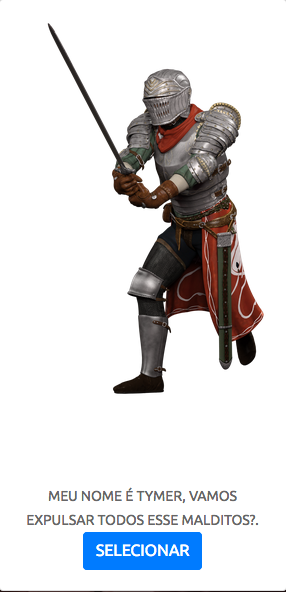
\includegraphics[keepaspectratio=true,scale=0.6]{figuras/tymer.png}
	\caption{Personagem Tymer}
	Fonte: Autor
	\label{tymer}
\end{figure}
\clearpage
\subsubsection{Scar}
\begin{figure}[h]
	\centering
	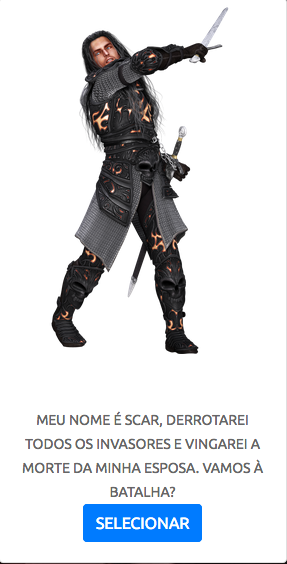
\includegraphics[keepaspectratio=true,scale=0.6]{figuras/scar.png}
	\caption{Personagem Scar}
	Fonte: Autor
	\label{scar}
\end{figure}

\subsection{Questões}
Existem diferentes tipos de questões que podem ser solucionados pelo jogador. A correção destas, são feitas automaticamente
pelo sistema de acordo com respostas pré cadastradas na base de dados.

Os  tipos de questões são:

\begin{itemize}
	\item Verdadeiro ou falso;
	\item Lacunas;
	\item Múltipla escolha
\end{itemize}

Cada resposta contabilizada como correta, são adicionados 10 pontos à pontuação total do jogador. Não há limites de tentativas
de solucionar as questões.

Para cada tentativa de resposta julgada como incorreta, é apresentado a alternativa correta para aquela questão.

\subsection{\textit{Levels}}

A medida que o jogador conquista maiores pontuações, é desbloqueado o novo level que consiste na liberação de novos conteúdos 
mais avançados em relação aos anteriores.  No total, existem 12  levels, os  conteúdos abordados em cada um deles são apresentado 
logo a seguir.

\begin{table}[h]
	\centering
	\resizebox{.5\textwidth}{!}{%
	\begin{tabular}{|l|l|l|l|}
	\hline
	\textbf{\textit{Level}} & \textbf{Conteúdo} \\ \hline
	01 & Algoritmos \\ \hline
	02 & Linguagem de Programação \\ \hline
	03 & Tipos de dados \\ \hline
	04 & Entrada e saída de dados \\ \hline
	05 & Operações primitivas \\ \hline
	06 & Variáveis e expressões \\ \hline
	07 & Estruturas de decisão \\ \hline
	08 & Laços de repetição \\ \hline
	09 & Vetores \\ \hline
	10 & Matrizes \\ \hline
	11 & Funções e Procedimentos \\ \hline
	12 & Arquivos \\ \hline
	\end{tabular}%
	}
	\caption{Conteúdos por \textit{level}}
	Fonte: {Autor}
	% \small{Quadro 2 - Requisitos funcionais} 
\end{table}

Os levels são compostos por questões, como as apresentadas na seção anterior.

\subsection{Desafios}

\subsubsection{Jogador contra Jogador}
A ferramenta dedica um módulo inteiramente voltado para que jogadores possam desafiar outros jogadores, os
desafios podem variar de simples perguntas até implementação de pequenos códigos que, após solucionados, devem
ser avaliados pelo jogador/aluno desafiante. Ambos os jogadores são recompensados pela interação de eleborar, responder
e avaliar os desafios.


\subsubsection{Desafio individual}
Os desafios individuais consistem em resolver diferentes tipos de  desafios pré cadastrados no sistema que, uma vez 
solucionados e avaliados pelo administrador do sistema e, tendo sido julgado por este como correto, é adicionado à
pontuação total do jogador mais 100 pontos. Os  desafios variam de simples respostas até implementação de códigos.


\section{Teste: Experiência de uso}

Com objetivo levantar informações a respeito da experiência de uso dos jogadores. Foi elaborado e aplicado um questionário 
onde os participantes responderam algumas perguntas de como foi a experiência de uso da ferramenta, interface e etc. Participaram da pesquisa
cerca de 15 alunos dos diversos cursos de engenharias da FGA.

Nesta sessão, são apresentados algumas análises realizadas em cima dos dados obtidos por meio do questionário.

Como mencionado anteriormente, participaram da experiëncia cerca de 15 alunos com idades variando de 18 à 36 anos. 
Aproximadamente 93,3\% (cerca de 14 alunos) dos participantes são homens, 86,7\% (cerca de 13 alunos) já cursaram alguma
disciplina introdutória de programação.

Além de perguntas relacionadas à orientação sexual, idade e se já cursaram alguma disciplina introdutória de programação.
Foram elaboradas questões a respeito da experiênciade de uso dos jogadores/alunos. Na tabela \ref{exp}, são apresentadas 
o percentual de respostas para as afirmativas, que podiam ser julgadas em uma escala de variação de 1 à 5.

\begin{table}[h]
	\centering
	\resizebox{0.9\textwidth}{!}{%
	\begin{tabular}{|p{5cm}|p{3cm}|p{3cm}|p{3cm}|p{3cm}|p{3cm}|}
	\hline
	\textbf{Afirmativa} & \textbf{(1) Discordo totalmente } & \textbf{(2) Discordo parcialmente} & \textbf{(3) Não concordo nem discordo} & \textbf{(4) Concordo parcialmente} & \textbf{(5) Concordo totalmente}  \\ \hline
	1. Com relação à temática, narrativa e personagens da ferramenta eles são considerados atraentes. & 0\% & 0\% & 6,7\% & 13,3\% & 80\%  \\ \hline
	2. Com relação aos aspectos de Layout e aparência visual são de boa qualidade &0\% &0\% & 6,7\% & 26,7\% & 66,7\%  \\ \hline
	3. O site não está poluído visualmente & 6,7\% & 6,7\% & 0\% & 6,7\% & 80\% \\ \hline
	4. O site é confuso & 60\% & 20\% & 0\% & 0\% & 20\% \\ \hline
	5. O site é de fácil navegação & 0\%& 6,7\% & 0\% & 26,7\% & 66,7\% \\ \hline
	6. O site é de fácil de utilização & 0\% & 6,7\% & 6,7\% & 20\% & 66,7\% \\ \hline
	7. O site é agradável & 0\% & 0\% & 0\% & 33,3\% & 66,7\%\\ \hline
	8. O site apresenta fácil entendimento das informações & 0\% & 0\% & 0\% & 26,7\% & 73,3\% \\ \hline
	9. Eu utilizaria ou recomendaria o uso da ferramenta para o propósito que ele foi construído. & 0\% & 0\% & 0\% & 26,7\% & 73,3\% \\ \hline
	10. A partir da experiência ao utilizar o ProGame eu me considero pelnamente satisfeito. & 0\% & 0\% & 0\% & 46,7\% & 53,3\%\\ \hline
	\end{tabular}%
	}
	\caption{Teste de usabilidade}
	\label{exp}
	Fonte: {Autor}
	% \small{Quadro 2 - Requisitos funcionais} 
\end{table}

O questionário aplicado pode ser apreciado no apêndice \ref{apenda} deste trabalho.

\section{Repositórios}

Conforme apresentado neste trabalho, a aplicação e seu banco de dados foram hospedados no servidor Heroku e 
pode ser acessada por meio do endereço apresentado a seguir.

\begin{itemize}
	\item Servidor da aplicação: https://progamefication.herokuapp.com/
	\item Versionamento de código: https://github.com/Eduardojvr/ProGame-PG
\end{itemize}


